\documentclass{beamer}

\mode<presentation>
\usepackage{beamerthemesplit}
\usepackage[latin1]{inputenc}
\usepackage{amsmath}
\usepackage{amsfonts}
\usepackage{amssymb}
\usepackage{makeidx}
\usepackage{graphicx}
\usepackage{float}
\usepackage{color}
\usepackage{multirow}
\usepackage{amsmath,amsthm,amssymb}
\usepackage{subfigure}
\usepackage[german]{babel}
\usepackage{xy}

\usetheme{antibes}
\setbeamertemplate{footline}[page number]{}
\title{Implementation of Nine Men`s Morris}
\author{Lars Engel \newline Vikash \newline Ahsan Yousuf}

\institute{Fachhochschule Kiel}
\date{\today}

\newcommand\Wider[2][1.9cm]{%
\makebox[\linewidth][c]{%
  \begin{minipage}{\dimexpr\textwidth+#1\relax}
  \raggedright#2
  \end{minipage}%
  }%
}

\begin{document}

\AtBeginSection[]
{
	\begin{frame}
	\footnotesize{
		\frametitle{Outline}
		\tableofcontents[currentsection]}
	\end{frame}
}

\begin{frame}
\titlepage
\end{frame}


\section{Introduction}
\begin{frame}{Introduction }
\begin{itemize}
\item KUKA lbr iiwa 7.
\item Game called Nine Men's Morris.
\item Cognex Camera.
\item Artificial Intelligence.
\end{itemize}
\end{frame}

\section{Milestones of Project}
\begin{frame}{Milestones of the Project}
\begin{itemize}
\item Human vs KUKA robot.  
\item Robot can detect human moves and can perform its own moves wisely.
\item Robot knows its turn after human.
\item Through a camera robot interacts with real world.
\end{itemize}
\end{frame}

\section{Software and Hardware Tools}
\begin{frame}{Software and Hardware Tools}
\begin{itemize}
\item Robotic Arm LBR iiwa 7 R800 1 by KUKA Laboratories.
\begin{itemize}
\item Sunrise Workbench.
\end{itemize}
\item Cognex IS 7000 Camera.
\begin{itemize}
\item Cognex In-Sight Explorer.
\end{itemize}
\vspace{\baselineskip}
\item Eclipse IDE for testing AI and Modbus TCP/IP Connection.
\item GIT for version control.
\end{itemize}
\end{frame}

\section{Workflow}
\subsection{Basic requirements to achieve target}
\begin{frame}{Basic requirements to achieve target}
\begin{itemize}
\item Understanding of Nine Men's Morris games rules.
\item Getting started with some useful methods of the robot.
\item Learn how to use the Camera. 
\end{itemize}
\end{frame}


\subsection{Main User Stories}
\begin{frame}{Main User Stories}
\Wider{
\begin{figure}[h!]
  	\centering
	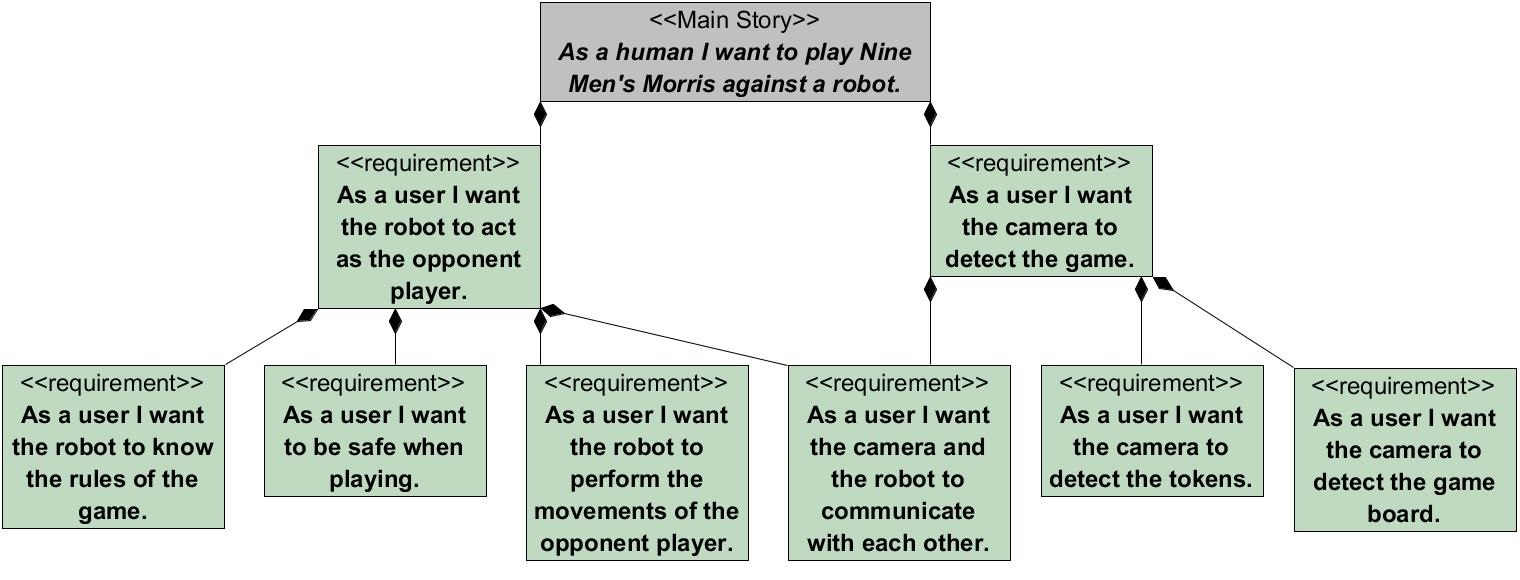
\includegraphics[width=12.5cm]{imgs/stories.jpg}
\end{figure}
}
\end{frame}



\section{Implementation phase}
\subsection{Program Architecture}
\begin{frame}{Program Architecture}
\Wider{
\begin{figure}[h!]
  	\centering
  	\tiny{Class Diagram}
	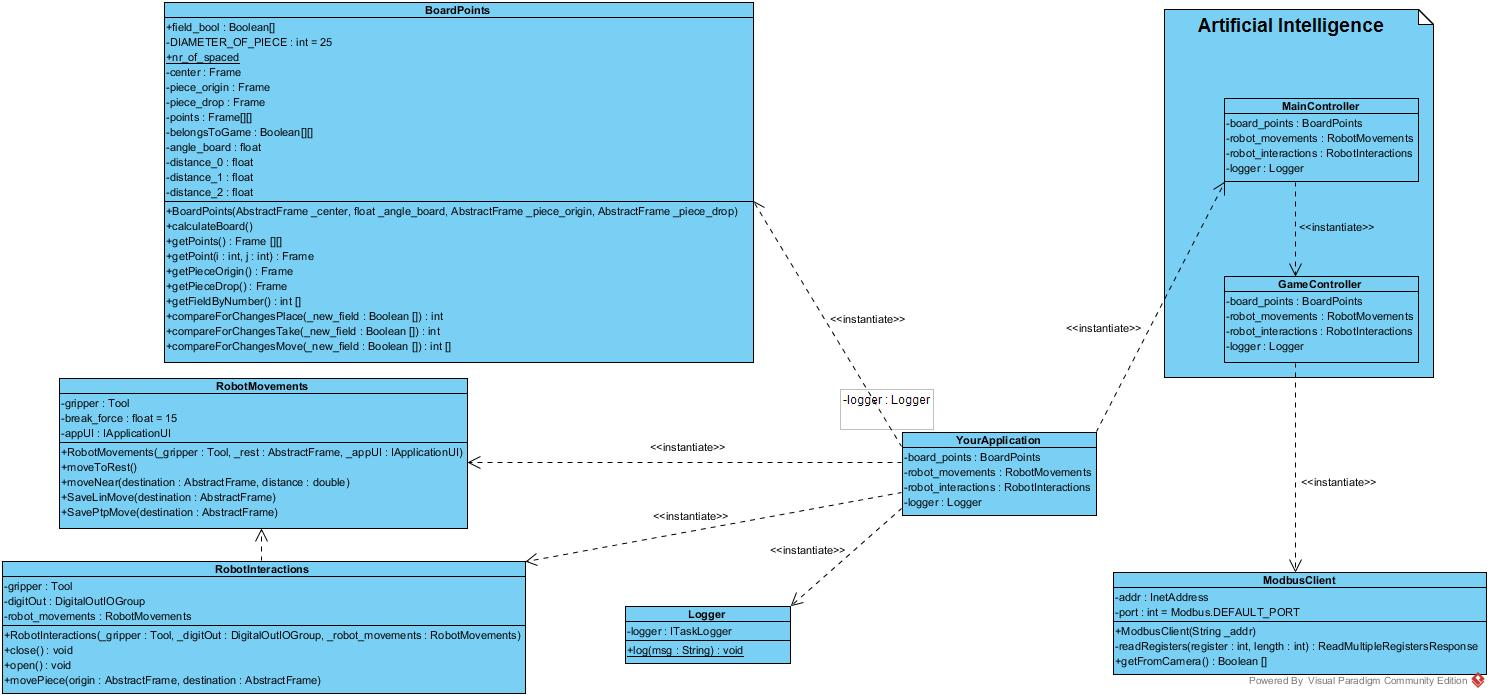
\includegraphics[width=12.5cm]{imgs/classDiagram.jpg}
\end{figure}
}
\end{frame}

\subsection{Safety}
\begin{frame}{Safety}
\Wider{
\begin{figure}[h!]
	\tiny{Listing 1: Extract from the Class RobotMovements}\\
  	\centering
  	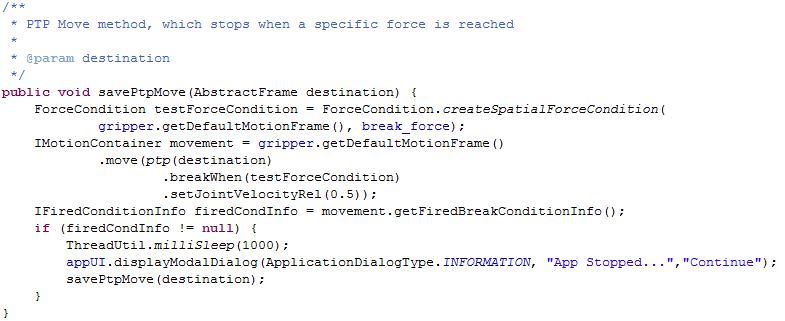
\includegraphics[width=12.4cm]{imgs/safety.png}
\end{figure}
}
\Wider{
\begin{figure}[h!]
  	\centering
  	\tiny{Listing 2: Call for save PTP Movement Method}
	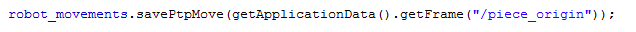
\includegraphics[width=10cm]{imgs/safety_02.png}
\end{figure}
}
\end{frame}

\subsection{Visual Analysis}
\begin{frame}{Visual Analysis}
\Wider{
\begin{figure}[h!]
  	\centering
	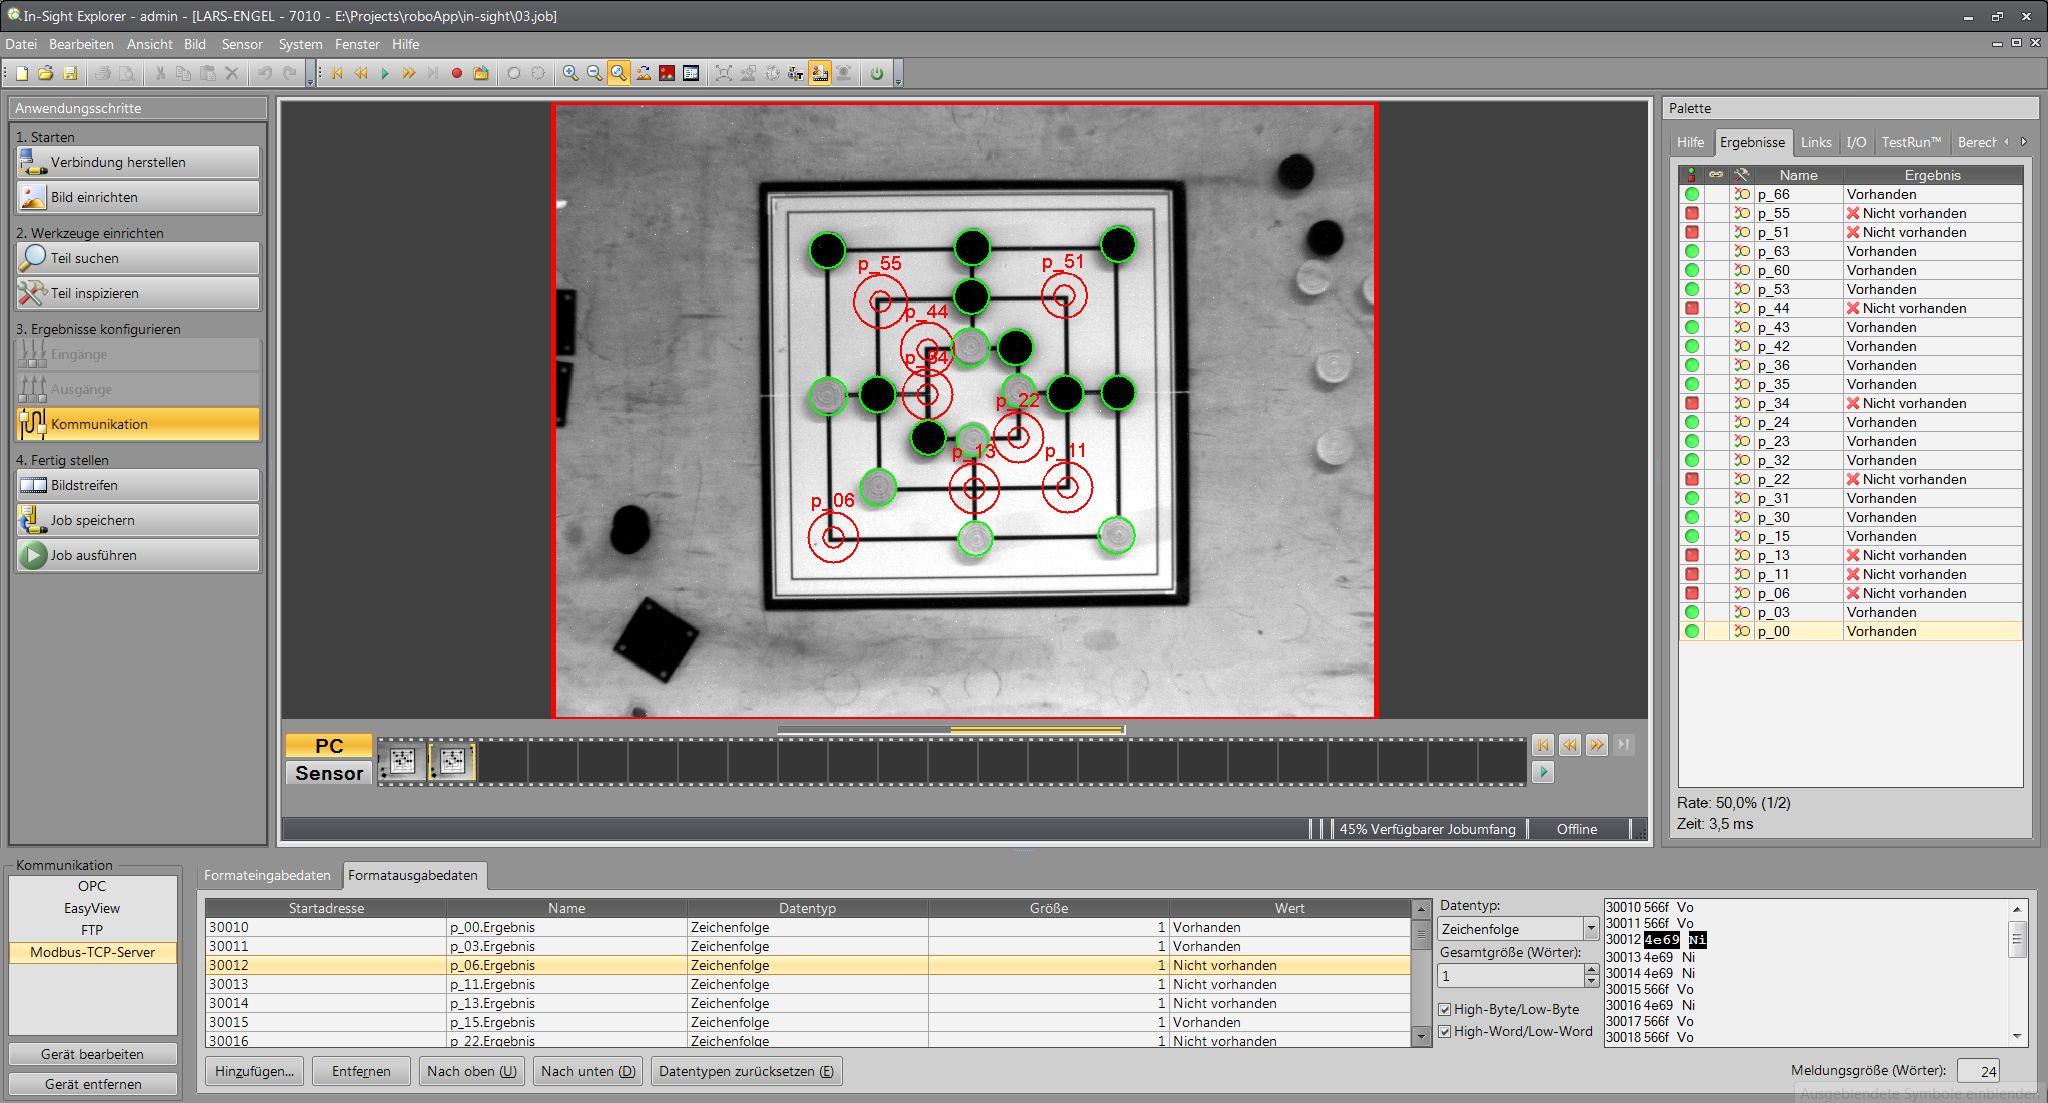
\includegraphics[width=12.5cm]{imgs/camera.png}
\end{figure}
}
\end{frame}
\subsection{Communication between Robot and Camera}
\begin{frame}{Communication between Robot and Camera}

\end{frame}

\section{Difficulties faced}
\begin{frame}{Difficulties faced during the project}
\begin{itemize}
\item Understanding of robotics
\begin{itemize}
\item Robot movement limitations
\item Coordination transformations
\end{itemize}
\item Understanding of AI.
\item Recognition by the camera.
\begin{itemize}
\item Game board alignment.
\item Token recognition
\end{itemize}
\item Communication of robot and camera.
\end{itemize}
\end{frame}


\section{Conclusion}
\begin{frame}{Conclusion}
\begin{itemize}
\item Human can play Nine Men's Morris against the robot.
\item Possible Improvements:
\begin{enumerate}
\item Better cheat handling
\item Board orientation and location
\item Choosing token color and starting player
\end{enumerate}
\end{itemize}
\end{frame}


\begin{frame}
\begin{center}  
\Huge \textbf{ThankYou}
\end{center}
\end{frame}

\end{document}

